%%%%%%%%%%%%%%%%%%%%%%%%%%%%%%%%%%%%%%%%%
% Tufte-Style Book (Minimal Template)
% LaTeX Template
% Version 1.0 (5/1/13)
%
% This template has been downloaded from:
% http://www.LaTeXTemplates.com
%
% License:
% CC BY-NC-SA 3.0 (http://creativecommons.org/licenses/by-nc-sa/3.0/)
%
% IMPORTANT NOTE:
% In addition to running BibTeX to compile the reference list from the .bib
% file, you will need to run MakeIndex to compile the index at the end of the
% document.
%
%%%%%%%%%%%%%%%%%%%%%%%%%%%%%%%%%%%%%%%%%

%----------------------------------------------------------------------------------------
%	PACKAGES AND OTHER DOCUMENT CONFIGURATIONS
%----------------------------------------------------------------------------------------

\documentclass{tufte-book} % Use the tufte-book class which in turn uses the tufte-common class

\hypersetup{colorlinks} % Comment this line if you don't wish to have colored links

% hybrid automata definition
\newcommand{\A}{\mathcal{A}}
\newcommand{\D}{\mathcal{D}}
\newcommand{\T}{\mathcal{T}}
%\newcommand{\S}{\mathcal{S}}

\newcommand{\booleans}{{\mathbb{B}}}
\newcommand{\reals}{{\mathbb{R}}}
\newcommand{\naturals}{{\mathbb{N}}}

\newcommand{\val}[1]{{\mathit{val}(#1)}}
\newcommand{\guard}{{\mathit{guard}}}
\newcommand{\reset}{{\mathit{reset}}}
\newcommand{\hyxml}{{{\sf HyXML}\xspace}}

\newcommand{\ccee}{{{\mathsf C2E2}}}
%\newcommand{$\ccee$}{{{\sf $\ccee$}}}


% comments
\newcommand{\sayan}[1]{{\textcolor{blue}{#1}}}

\usepackage{microtype} % Improves character and word spacing

\usepackage{lipsum} % Inserts dummy text

\usepackage{booktabs} % Better horizontal rules in tables

\usepackage{pgf} % classes for drawing diagrams
\usepackage{tikz}
\usepackage[utf8]{inputenc}
\usetikzlibrary{arrows,automata}
\usetikzlibrary{positioning}

\usepackage{graphicx} % Needed to insert images into the document
\graphicspath{{graphics/}} % Sets the default location of pictures
\setkeys{Gin}{width=\linewidth,totalheight=\textheight,keepaspectratio} % Improves figure scaling

\usepackage{fancyvrb} % Allows customization of verbatim environments
\fvset{fontsize=\normalsize} % The font size of all verbatim text can be changed here

\newcommand{\hangp}[1]{\makebox[0pt][r]{(}#1\makebox[0pt][l]{)}} % New command to create parentheses around text in tables which take up no horizontal space - this improves column spacing
\newcommand{\hangstar}{\makebox[0pt][l]{*}} % New command to create asterisks in tables which take up no horizontal space - this improves column spacing

\usepackage{xspace} % Used for printing a trailing space better than using a tilde (~) using the \xspace command

\newcommand{\monthyear}{\ifcase\month\or January\or February\or March\or April\or May\or June\or July\or August\or September\or October\or November\or December\fi\space\number\year} % A command to print the current month and year


\newcommand{\openepigraph}[2]{ % This block sets up a command for printing an epigraph with 2 arguments - the quote and the author
\begin{fullwidth}
\sffamily\large
\begin{doublespace}
\noindent\allcaps{#1}\\ % The quote
\noindent\allcaps{#2} % The author
\end{doublespace}
\end{fullwidth}
}

\newcommand{\blankpage}{\newpage\hbox{}\thispagestyle{empty}\newpage} % Command to insert a blank page


\usepackage{makeidx} % Used to generate the index
\makeindex % Generate the index which is printed at the end of the document

\usepackage{subfig}  % LMB Used to add subfigures

%----------------------------------------------------------------------------------------
%	BOOK META-INFORMATION
%----------------------------------------------------------------------------------------



\usepackage{xcolor}

\def\chpcolor{blue!45}
\def\chpcolortxt{blue!60}
\def\sectionfont{\sffamily\LARGE}

\setcounter{secnumdepth}{2}

\makeatletter
%Section:
\def\@sectionstrut{\vrule\@width\z@\@height12.5\p@}
\def\@makesectionhead#1{%
  {\par\vspace{20pt}%
   \parindent 0pt\raggedleft\sectionfont
   \colorbox{\chpcolor}{%
     \parbox[t]{90pt}{\color{white}\@sectionstrut\@depth4.5\p@\hfill
       \ifnum\c@secnumdepth>\z@\thesection\fi}%
   }%
   \begin{minipage}[t]{\dimexpr\textwidth-90pt-2\fboxsep\relax}
   \color{\chpcolortxt}\@sectionstrut\hspace{5pt}#1
   \end{minipage}\par
   \vspace{10pt}%
  }
}
\def\section{\@afterindentfalse\secdef\@section\@ssection}
\def\@section[#1]#2{%
  \ifnum\c@secnumdepth>\m@ne
    \refstepcounter{section}%
    \addcontentsline{toc}{section}{\protect\numberline{\thesection}#1}%
  \else
    \phantomsection
    \addcontentsline{toc}{section}{#1}%
  \fi
  \sectionmark{#1}%
  \if@twocolumn
    \@topnewpage[\@makesectionhead{#2}]%
  \else
    \@makesectionhead{#2}\@afterheading
  \fi
}
\def\@ssection#1{%
  \if@twocolumn
    \@topnewpage[\@makesectionhead{#1}]%
  \else
    \@makesectionhead{#1}\@afterheading
  \fi
}
\makeatother

%%% XML


\usepackage{listings}

\usepackage{color}
\definecolor{gray}{rgb}{0.4,0.4,0.4}
\definecolor{darkblue}{rgb}{0.0,0.0,0.6}
\definecolor{cyan}{rgb}{0.0,0.6,0.6}

\lstset{
  basicstyle=\ttfamily,
  columns=fullflexible,
  showstringspaces=false,
  commentstyle=\color{gray}\upshape
}

\lstdefinelanguage{XML}
{
  morestring=[b]",
  morestring=[s]{>}{<},
  morecomment=[s]{<?}{?>},
  stringstyle=\color{black},
  identifierstyle=\color{darkblue},
  keywordstyle=\color{cyan},
  morekeywords={xmlns,version,type}% list your attributes here
}

%%%%

\title{C2E2 User's Guide\\ \large{Ver 2.1 \ \ December 2020}} % Title of the book
\author{\href{http://publish.illinois.edu/c2e2-tool/}{C2E2 Team} \\ \href{mailto:c2e2help@gmail.com}{c2e2help@gmail.com}}
% % Author

\publisher{University of Illinois at Urbana-Champaign} % Publisher

%----------------------------------------------------------------------------------------

\begin{document}

\frontmatter

\vbox{
	\centering
	\maketitle %this typesets the contents of \title,
	\vspace{2cm} 
		
\includegraphics[width=1.5\textwidth]{Figures/c2e2v2logo}
%	\author and \date
}

%----------------------------------------------------------------------------------------
%	EPIGRAPH
%----------------------------------------------------------------------------------------

%\thispagestyle{empty}
%\openepigraph{Quotation 1}{Author, {\itshape Source}}


%----------------------------------------------------------------------------------------

%\maketitle % Print the title page

%----------------------------------------------------------------------------------------
%	COPYRIGHT PAGE
%----------------------------------------------------------------------------------------

\newpage
\begin{fullwidth}
~\vfill
\thispagestyle{empty}
\setlength{\parindent}{0pt}
\setlength{\parskip}{\baselineskip}
Copyright \copyright\ \the\year\ \thanklessauthor

%\par\smallcaps{Published by \thanklesspublisher}

%\par\smallcaps{\url{http://www.bookwebsite.com}}

%\par License information.\index{license}

\par\textit{Compiled on \today}
\end{fullwidth}

%----------------------------------------------------------------------------------------

\tableofcontents % Print the table of contents





\mainmatter

\chapter{Acknowledgements}
\label{sec:ack}

\paragraph{Authors and Contributors.}
Lucas Brown $\circ$
Zongnan Bao $\circ$
Chuchu Fan $\circ$
Parasara Sridhar Duggirala $\circ$
Suket Karnawat $\circ$
Yangge Li $\circ$
Yu Meng $\circ$
Sayan Mitra $\circ$
Matthew Potok $\circ$
Bolun Qi $\circ$
Mahesh Viswanathan 
%Zhenqi Huang $\circ$
%Taylor Johnson $\circ$ 
%Karthikeyan Manamcheri Sukumar $\circ$
%Le Wang $\circ$

\paragraph{Supported by}
Department of Computer Science and Department of Electrical and Computer Engineering at the University of Illinois at Urbana Champaign $\circ$
Coordinated Science Laboratory $\circ$
The National Science Foundation $\circ$ 
Air Force's Office of Scientific Research.



\chapter{Introduction}
\label{sec:intro}
$\ccee$ is a tool for verifying time-bounded invariant properties of hybrid automata models. It supports models with nonlinear dynamics, discrete transitions, and sets of initial states. The invariant properties have to be specified by conjunctions of linear inequalities. Internally, $\ccee$ implements the simulation-based verification algorithms described in the sequence of publications~\citet{fan2016automatic,ChuchuATVA,DMV13,DuggiralaWMVM14,SM:HSCC2011}. The new version of $\ccee$ uses an on-the-fly discrepancy computation algorithm \citet{ChuchuATVA} to automatically generate neighborhoods that conservatively contain all the behaviors of neighboring trajectories. In a nutshell, $\ccee$ parses and transforms the hybrid automata model to a mathematical representation, it generates faithful numerical simulations of this model using a validated numerical simulator, it then bloats these simulations using on-the-fly discrepancy computation to construct over-approximations of the bounded time reachable set, and it iteratively refines these over-approximations to prove the invariant or announce candidate counterexamples.
%In a nutshell, it parses and transforms the  Stateflow\textsuperscript{TM} model to a mathematical representation, it generates faithful numerical simulations of this model using a validated numerical simulator, it then bloats these simulations using user-provided annotations  to construct over-approximations of the bounded time reachable set, and it iteratively refines these over-approximations to prove the invariant or announce candidate counterexamples. 

$\ccee$ has a GUI for loading and editing of hybrid automata models and properties in an internal $\hyxml$ format, launching the verifier, and for plotting 2D sections of the reach set computed by the verifier. 

Please contact us at \href{mailto:c2e2help@gmail.com}{c2e2help@gmail.com} and let us know about your experiences using $\ccee$. 
Previous versions of $\ccee$ allowed for the editing of Stateflow\textsuperscript{TM} models and readily supported numerical simulators like {\sf VNODE-LP}~\citet{vnode2006}. Some of these features are getting depreciated because of numerical instability, lack of support, etc. Let us know if you are interested in these features. 

\chapter{Installation}
\label{chap:install}
%Example .hyxml files are included and located in the \texttt{examples} folder. 

\section{Supported platforms}
$\ccee$ has been tested on different versions of Ubuntu, including  Ubuntu 16.04, 64-bit. With a little extra work, 

If you are using a different OS, we recommend that you download the virtual machine instead.

\section{Download and install $\ccee$}
\begin{itemize}
\item Download the latest distribution of $\ccee$ distribution from:
\url{http://publish.illinois.edu/c2e2-tool/download/}.
\item Unzip the files in a local directory, say \texttt{\textasciitilde/c2e2/}. \linebreak
\texttt{tar -xvzf c2e2-2.0.0.tar.gz -C \textasciitilde/c2e2/}
\item  Navigate to that directory and run installRequirements.sh with superuser privileges. This should install all the packages needed and may take a while. \linebreak
\texttt{cd \textasciitilde/$\ccee$/} \linebreak
\texttt{sudo ./installRequirements.sh}  
\item Launch the GUI for loading, editing, and verifying models. \linebreak
\texttt{./runc2e2}
\item If any of the above steps fail then you can try to install the packaged listed in the file \texttt{installRequirements} separately. 
\end{itemize}
%The list of all the needed packages are given in Appendix~\ref{app:packs}. 

%\section{Install the Virtual Machine}
%The virtual machine can be download from \url{http://publish.illinois.edu/c2e2-tool/download/}. Oracle VM VirtualBox was used to create and test the Open Virtual Appliance (.ova). 
%% \item If any of the above steps fail, you have the second option to download a virtual machine running 64 bit Ubuntu 16.04 (password: $\ccee$) that has the newest version of $\ccee$ already installed. Oracle VM VirtualBox was used to create the Open Virtual Appliance (.ova), though it should work properly on other virtualization applications that can load .ova files.
%% \item Examples in form of \texttt{.hyxml} files are in included in the  \texttt{Examples} folder. 
%% \item Errors and warnings are logged in \texttt{/work-dir/warnings}
%%Check out the updates on our website\footnote{https://publish.illinois.edu/$\ccee$-tool/} for further information to support Matlab Stateflow model (\texttt{.mdl}) files.
%\end{itemize}

% \begin{itemize}
% \item $\ccee$ is already installed in the virtual machine image for the Artifact Evaluation.

% \item {\bf Disclaimer:} this artifact evaluation submission (the \texttt{.ova} file) is generated using VM Workstation Player and might have some issues with VirtualBox.
% \end{itemize}

% $\ccee$ can also be installed on Mac.
% Instead of using the installation scripts, the packages will have to be manually installed with the help of brew (\url{http://brew.sh/}) and pip. If you do not already have brew, install it as directed by the website.
% \begin{itemize}
% \item Using "brew install <package-name>", install python, gmp, ppl, pygtk, gnuplot, boost, swig.
% \item Using "pip install <package-name>", install psutil, sympy, lxml. If lxml fails install command line developer tools by running "xcode-select --install" and then try again.
% \item Run installGLPK. If you run into errors, refer to this \href{http://hichenwang.blogspot.com/2011/08/fw-installing-glpk-on-mac.html}{guide}.
% \item Install PyGLPK by using this \href{http://blog.ducky.io/python/2013/07/01/Installing-Python-glpk}{guide} with slight modifications. DO NOT install GLPK using home-brew and install ply version 3.4 by running "pip install ply==3.4".
% \item Install GnuPlot by downloading the zip \href{http://gnuplot-py.sourceforge.net/}{here} and running "python setup.py install".
% \item Finally run "mkdir -p ~/.local/share/". You should now have all the dependencies and the program should run smoothly.
% \end{itemize}


\section{Older Versions}
Earlier versions of $\ccee$ are archived at:
\url{http://publish.illinois.edu/c2e2-tool/download/}
Tar-zipped source files and virtual machines are available. From version 2.1 onward the source files are made available from github.



\chapter{Key Improvements in Version 2.1}

Version 2.1 of $\ccee$ is the first version to be released as open source software. There are several other important bug fixes and a more expanded support for command-line usage.

$\ccee$ version 2.0 improved the usability significantly. Previously, editing $\hyxml$ models had to be done using an external text editor outside of $\ccee$. This prolonged the editing-parsing-debugging cycle. To fix this, we made two significant updates to our GUI:
\label{version}
\begin{itemize}
\item Models are now editable directly from the GUI on the \emph{Model} tab.
\item The new \emph{Editor} tab allows you to edit the $\hyxml$ directly without closing $\ccee$
\end{itemize}

The \emph{Plot} tab has been updated to improve usability and flexibility:
\begin{itemize}
\item The plotter now creates an interactive HTML.
\item Any data file generated by $\ccee$ can be loaded into the plotter at any time. 
\end{itemize}

\chapter{Getting Started}
\label{start}

In this chapter, we give a quick tour of some features of $\ccee$ using one of the examples that are distributed as part of the package. 
%In Chapter~\ref{models} we will describe creation of new Stateflow\textsuperscript{TM} models.

\section{Opening a Model}
\label{sec:open}
In the $\ccee$ folder, type the command \texttt{./run$\ccee$} to launch $\ccee$ and you should be able to see the front end of the tool as Figure~\ref{figure:frontend}. Once $\ccee$ is launched, go ahead and open one of the examples from the \texttt{File} menu (or use \texttt{Ctrl + O}). All examples are stored in the \texttt{examples} folder inside \texttt{$\ccee$} folder. For this tutorial, we will use the model of an adaptive cruise control system (see the example webpage \footnote{https://publish.illinois.edu/$\ccee$-tool/example/adaptive-cruise-control/}) which is stored as \texttt{TotalMotion40s.hyxml}. For the description of other examples, please refer to the examples webpage \footnote{https://publish.illinois.edu/$\ccee$-tool/example/}. 

\begin{marginfigure}
\centerline{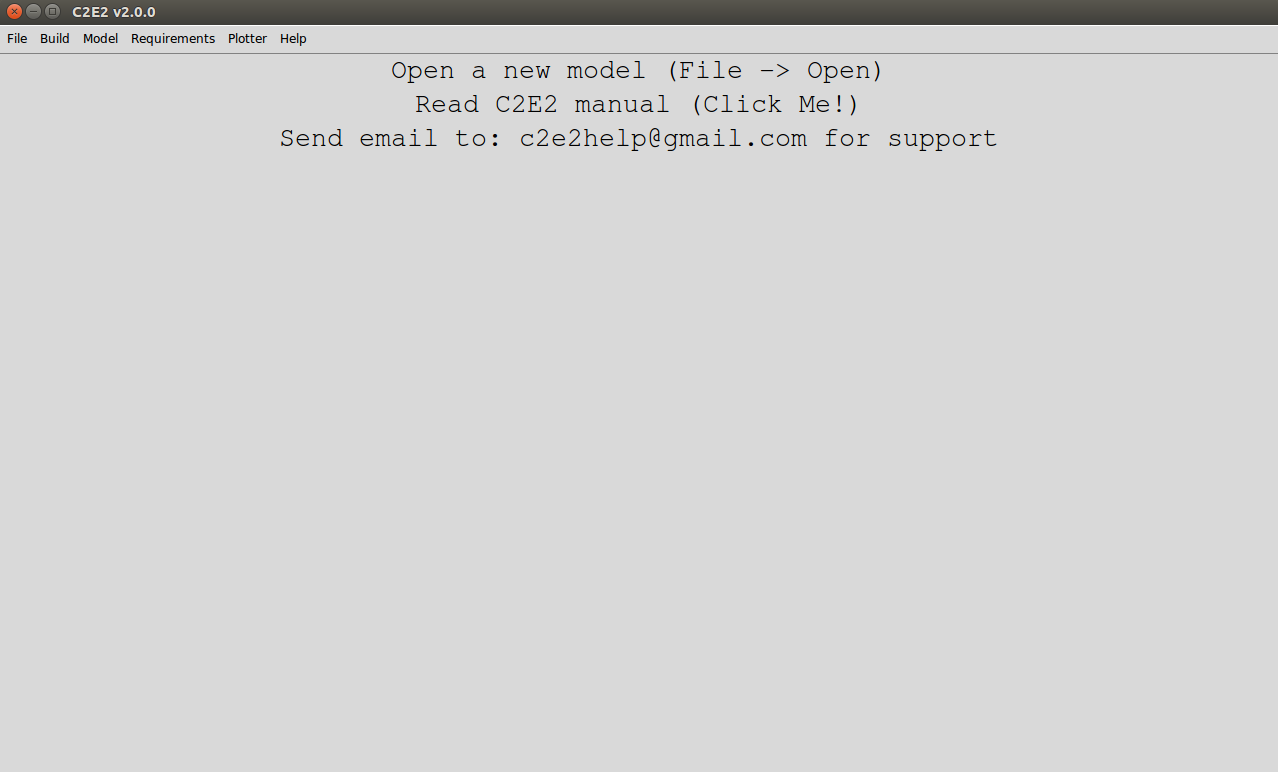
\includegraphics[scale=.24,keepaspectratio=true]{ManualImages/C2E2_version2.0/figure5-1.png}}
 \caption{Front end of $\ccee$ when launched} 
 \label{figure:frontend}
\end{marginfigure}

Upon opening the file , the $\ccee$ window should look similar to Figure~\ref{fig:parsetree}. The left hand side of this window is the hybrid automaton \emph{model tree} and the right hand side is the \emph{requirements sidebar}. 

\section{Model Tree}
When a model is opened, the $\hyxml$ is parsed and the result is displayed in the expandable \emph{model tree}. Automata are at the base, followed by Variables, Modes, and Transitions. Modes can further be expanded to display Flows and Invariants. Every item on the tree can be expanded to view details by clicking on the arrow to the left.
As you can see, our example in Figure~\ref{fig:parsetree} has five variables \emph{sx}, \emph{vx}, \emph{ax}, \emph{sy}, \emph{vy} and \emph{omega}. In addition, we have seven separate modes with six transitions between them. 


In version 2.0, you can now also edit the model directly from the \emph{model tree} by right-clicking the item you wish to edit, or by selecting it and using the options under the \emph{Build} menu. We will go over this in more detail in the next chapter.

\begin{figure}[h!]
\centerline{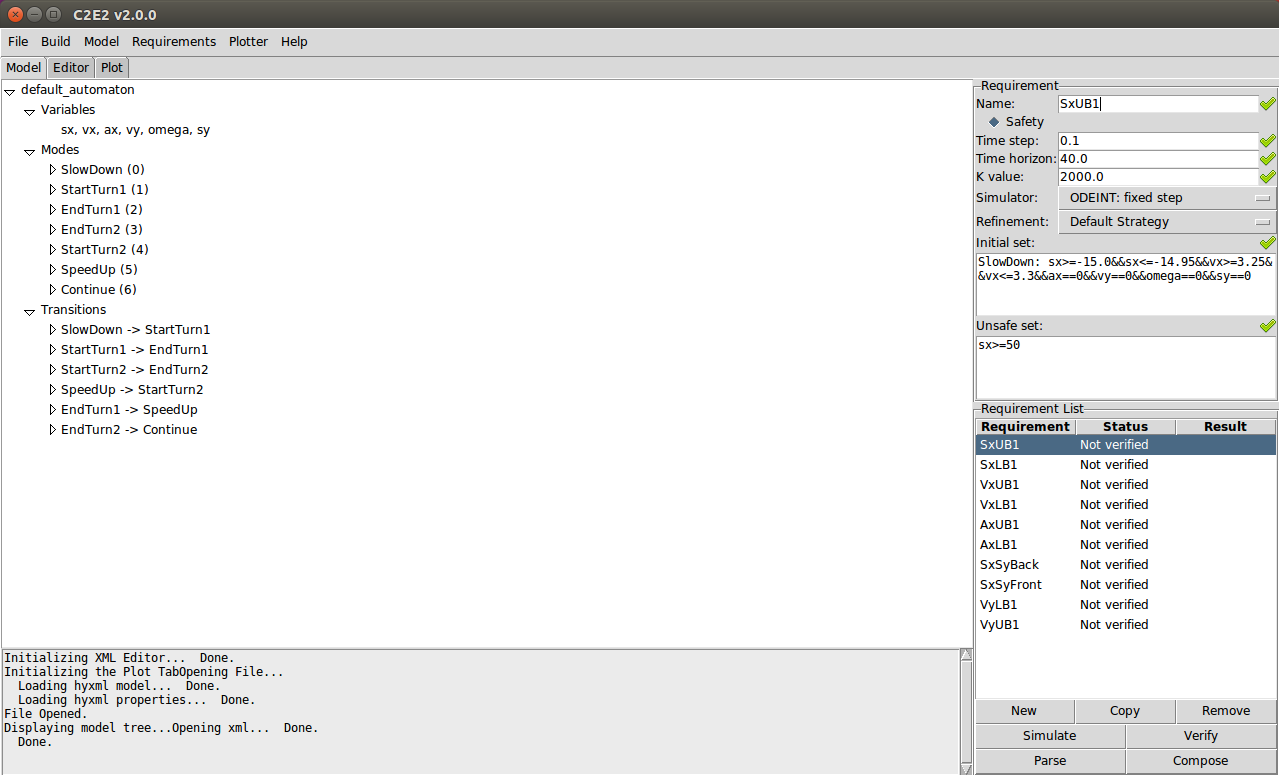
\includegraphics[scale=.22,keepaspectratio=true]{ManualImages/C2E2_version2.0/figure5-2.png}}
\caption{{\em Left:\/} Model parse tree. {\em Right:\/} Verification pane.} 
\label{fig:parsetree}
\end{figure}

\section{Requirements Sidebar}\label{sec:properties}
The lower part of the sidebar shows a list of requirements (properties) for the hybrid automaton that can be verified. The top part of the sidebar shows the detailed parameters of the highlighted requirement. Each requirement is a bounded time safety property.

\begin{itemize}
    \item{\em Name}\\ 
    Each requirement (property) to be checked is given a name. This name is used to name output files containing the reachtubes.
    \item{\em Time Horizon}\\
    The time bound for simulation and verification. 
    \item{\em Time Step}\\
    The time step-size used for simulation and verification. If adaptive step size is used for simulation (see below) then this value is ignored.  
    \item{\em K Value}\\
    The coordinate transformation step $K$ for nonlinear models has been set to $2000$ by default at the top right corner of the verification pane. This value is important since the inappropriate $K$ value will influence the final result. The user can change the $K$ value to see different outputs.
    \item {\em Simulator}\\
    Current version of $\ccee$ supports Odeint constant time step simulator and Odeint adaptive time step simulator. Previously, CAPD simulator was also supported, but no longer is in the current version. Please contact us if you wish to use the CAPD simulator. The default simulator is Odeint constant time step simulator, and it is been compiled when you opening the model. You can change the simulator by selecting different simulator from the simulator drop down menu as shown in Figure \ref{figure:simulator}. 

\begin{marginfigure}
\centerline{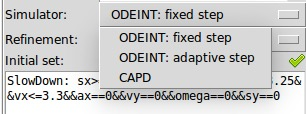
\includegraphics[scale=.24,keepaspectratio=true]{Figures/simulator.png}}
 \caption{Simulator drop down menu} 
 \label{figure:simulator}
\end{marginfigure}

    \item {\em Refinement}\\
    When the initial set needs refinement, $\ccee$ provides different refinement strategies. The default refinement strategy will refine the dimensions within the unsafe set for four times, then iteratively refine the dimension with the largest uncertainty size. $\ccee$ also supports user defined strategy, which can be found at Section~\ref{sec:refinement_defined}. To select the strategy, please use the drop down menu on GUI as shown in Figure \ref{figure:refine}.

\begin{marginfigure}
\centerline{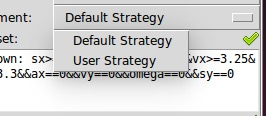
\includegraphics[scale=.24,keepaspectratio=true]{Figures/refine.png}}
 \caption{Refinement drop down menu} 
 \label{figure:refine}
\end{marginfigure}

\item \emph{Initial set}\\
    A linear predicate on the variables to specify the \emph{initial set} or \emph{starting states} on the \texttt{Initial set} textbox. Currently, the syntax for specifying the initial set is as follows:
    

 \item {\em Unsafe set}\\
    
  
\end{itemize}

%\section{Requirements}\label{sec:properties}

At the bottom of the \emph{requirement sidebar} is the \emph{requirement list}. 
This is where you can add, edit, copy properties and launch the verifier or simulator. 
Currently $\ccee$ verifies {\em bounded time linear invariant properties from linear bounded initial sets\/}.
Such properties are specified by the time bound ($T$), the initial set and the unsafe set. 
The {\em Time horizon\/} parameter listed at the top of the verification pane is the time bound.
%
Currently $\ccee$ requires both the initial and the unsafe sets to be described by a conjunction of linear inequalities involving the model variables.
The models in the \texttt{Examples} folder have already has a couple of sample properties.

\section{Creating a New Property}

Here we will walk you through the steps involved in creating a new property like in Figure~\ref{fig:property dialog}.


\begin{enumerate}
\item Click \texttt{New} in the property pane. This opens an empty new \texttt{Property} box on the Right panel in the middle for editing.
\item Enter a name for the property at the top, say \texttt{VxLB1}, in the first textbox.
\item Enter a linear predicate on the variables to specify the {\em initial set\/} or the {\em starting states\/} in the \texttt{Initial set} textbox. 
Currently, the syntax for specifying the initial set is as follows:\\
$\langle$ \texttt{mode-name} $\rangle$ : $\langle$ (\texttt{linear-inequality} \&\&)+ $\rangle$. \\
For example, for the above model: \\
\texttt{SlowDown}: sx>=-15.0 \&\& sx<=-14.95 
\&\& vx>=3.25 \&\& vx<=3.3 \&\& ax==0 \&\& vy==0
\&\& omega==0 \&\& sy==0  \\
is a valid expression for specifying the set of initial states. 
\item Enter the unsafe set in the \texttt{Unsafe set} textbox.
Currently, the syntax for specifying the unsafe set is a \&\&-separated sequence of linear inequalities:\\
vx<=2.1 
\item Press \texttt{Add}.
\end{enumerate}
%
\begin{marginfigure}
\centerline{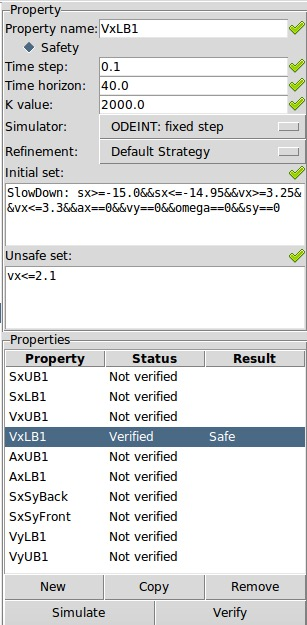
\includegraphics[width=\textwidth]{Figures/property_dialog.png}}
 \caption{Dialog box for adding properties checks the syntax of the initial and unsafe sets.}
 \label{fig:property dialog}
\end{marginfigure}
%
If all the expressions are syntactically acceptable then there will be little green checks
next to the textboxes and you will be able to save the property. Otherwise there will be a cross next to the textbox.
{\bf Both the unsafe set and the initial set should be described by a collection of linear inequalities and in addition the initial set should be bounded.\/}

Once the property is added the name of the property appears in the property pane. 
You may add several properties in the same way. 
You may also make copies of existing properties to save yourself some typing and edit them.
The added properties can be saved with the model. 
%See section~\ref{sec:loadsave}.

\section{Verifying}
\label{sec:verify}

Once you have created a model and added a property (see Section~\ref{sec:properties}) you can launch the verification engine by selecting the property and then clicking the \texttt{Verify} button.  


$\ccee$ is sound which means that you can trust the Safe/Unsafe answer proclaimed by it. 
In principle, $\ccee$ is also complete for robust properties~\citet{DMV13}. That is, if the 
model satisfies the property robustly\footnote{Robustness: the requirement that the actual reachable set of the model
does not skim the boundary of the unsafe set.}, and if the numerical precision supported by the 
algorithm is adequate then $\ccee$ should terminate with a Safe/Unsafe proclamation.
% 
In practice, the time it takes to verify is sensitive to the time horizon (T), the initial partition. 
You may want to first run the verification with small values of $T$ and initial set with small size.

The reachable set over-approximation computed by $\ccee$ is stored in the \texttt{/work-dir/<Requirement name>}. You can also check the log file at \texttt{/work-dir/log} to check the progress of the verification. Once the verification is done, the result (Safe/Unsafe/Unknown) will show up at the Result column (as in Figure~\ref{fig:safe}). Note that if you see verification result as \texttt{Unknown}, it is because of the following reason:
\begin{enumerate}
\item The system is neither robustly safe nor robustly unsafe~\citet{DMV13}.
\item Reachable set computed bloats up and thus the number of refinements needed is too large. Please go back and check the model dynamic and properties, or simulate first to see whether the system trajectories bloats up.
\end{enumerate}


%If you have multiple properties, then you may select one or more of them to be verified. Multiple properties are verified one at a time. When the verification is in progress clicking the \texttt{Abort} button aborts it.

\begin{marginfigure}
 \centerline{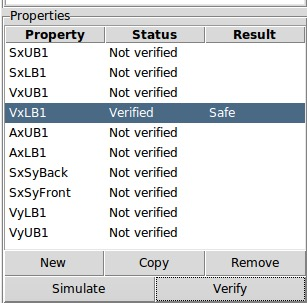
\includegraphics[scale=.25,keepaspectratio=true]{Figures/verified.png}}
 \caption{One or more properties can be selected by checking the boxes to the left of the property name. The \texttt{Verify} button launches the verification engine to verify one property at a time.} 
 \label{fig:safe}
\end{marginfigure}


\subsection{Simulation}
$\ccee$ also allows users to generate pure simulation traces from initial sets. Once you have created a model and added a property (see Section~\ref{sec:properties}) you can launch the simulation engine by selecting the property and then clicking the \texttt{Simulate} button. $\ccee$ will select several states from initial set and generate simulation traces from those initial states. Note the Safe/Unsafe result shown in this case only stands for the safety of the simulation traces instead of all the reachable states from the initial set.

\subsection{User defined refinement strategy}\label{sec:refinement_defined}
$\ccee$ supports user defined refinement strategy (see Section ~\ref{sec:open}). You can select USER DEFINE STRATEGY from the drop down menu as shown in Figure \ref{figure:refine}. In this case, you need to write down your strategy in a file named \texttt{refineorder.txt} and store it in the \texttt{/work-dir} folder. The file should be look like Figure \ref{figure:refine_file}. In each line, you should write down the index of the variables, the order of which is the same as the variables that are shown in the front end GUI. That is, "2`` means the second variable shown in the Variables list in the front end. Indexes that are larger than the dimension of system will be ignored automatically. $\ccee$ will refine the initial set according to the order written in \texttt{refineorder.txt} iteratively. For example, if use the refinement strategy as in Figure~\ref{figure:refine_file}, the dimension corresponding to the second variable will be refined three times, then the dimension corresponding to the first variable will be refined once, then go back to the first line of \texttt{refineorder.txt} if the verification process has not terminated.

\begin{marginfigure}
 \centerline{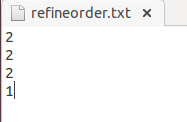
\includegraphics[scale=.25,keepaspectratio=true]{Figures/refine_order.png}}
 \caption{The user defined refine strategy file} 
  \label{figure:refine_file}
\end{marginfigure}


\subsection{Change Verified Properties}
Once a property is verified the status of the property will change to \texttt{Verified}, and the result \texttt{Safe/Unsafe/Unknown} will appear next to it. $\ccee$ will also create a new plot on the \emph{Plot Tab} for each verified property with the name $\langle$\texttt{property name}$\rangle$ \texttt{plot} (see Section~\ref{sec:plots}).  Once the result has shown up, if you change any of the parameters associated with the property, say the initial set or unsafe set, then the status of the property will change to \texttt{Verified*}. This (*) indicates that the property and parameters verified is outdated and you can launch the verifier again.

\chapter{Model ($\hyxml$) Creation and Editing}
\label{editor}



\begin{itemize}
\item The new text editor tab, brief overview of xml. refer to details given at the end of the manual. Screen shot of editor tab.
\item The graphical editing process. Variables, automata, transitions. Discuss all the dialog boxes. Screenshots. The error checks. 
\item Properties. New, copy, error checks.
\end{itemize}

\section{Editing in the GUI}
\label{sec:editing}

$\ccee$ version 2.0 allows editing directly in the GUI. To edit any item in the \emph{model tree}, simply right-click it or use the \emph{Model} menu in the menu bar. 

\subsection{Automata}
Automata are not edited as a whole, but rather they are edited by adding, editing, and removing the variables, modes, and transitions in the automaton. The automaton name can be edited through the \emph{Automaton} dialog. Similarly, when adding a new automaton, the name can be set in the same \emph{Automaton} dialog.
\begin{marginfigure}
 \centerline{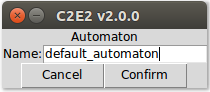
\includegraphics[scale=.25,keepaspectratio=true]{ManualImages/C2E2_version2.0/automaton-dialog.png}}
 \caption{Automaton Dialog} 
  \label{figure:automaton_dialog}
\end{marginfigure}
To add an automaton, right-click  the \emph{model tree} on an automaton name or in a blank area and select \emph{Add Automaton}. You can also add an automaton through the menu bar, \emph{Model} -> \emph{Automaton} -> \emph{Add Automaton}. 
To edit an automaton, the same procedures can be followed, however an automaton must be selected.


\subsection{Variables}
Variables are added, edited, and deleted through the \emph{Variable} dialog box. The \emph{Variable} dialog can be accessed through right-clicking the \emph{model tree} on the \emph{Variable} heading or on the variables themselves. It can also be accessed through the menu bar, \emph{Model} -> \emph{Variables} -> \emph{Edit Variables}. If you have two or more automata in the model, one of them must be selected. 
\begin{marginfigure}
 \centerline{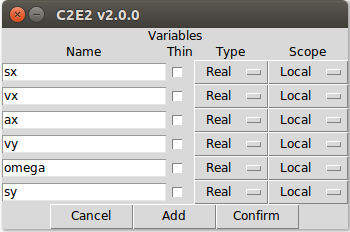
\includegraphics[scale=.25,keepaspectratio=true]{ManualImages/C2E2_version2.0/variables-dialog.png}}
 \caption{Variables Dialog} 
  \label{figure:variables_dialog}
\end{marginfigure}
Variables can be set as thin by selecting the check box next to their name. Variable type can be \emph{Real} or \emph{Integer}; variable scope can be \emph{Local}, \emph{Input}, or \emph{Output}.
To delete a variable, erase it's name and leave the field blank, then press \emph{Confirm}.

\subsection{Modes}
Modes are added, edited, and deleted through the \emph{Mode} dialog box. The dialog box is accessed through right-clicking the \emph{model tree} on the \emph{Mode} heading or the modes themselves. It can also be accessed through the menu bar, \emph{Model} -> \emph{Modes} -> \emph{Add Mode} or \emph{Edit Mode} or \emph{Delete Mode}.
\begin{marginfigure}
 \centerline{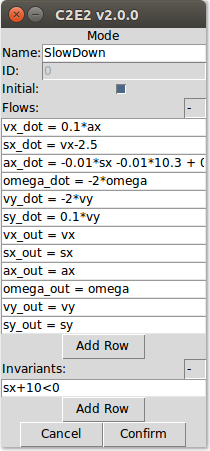
\includegraphics[scale=.25,keepaspectratio=true]{ManualImages/C2E2_version2.0/mode-dialog.png}}
 \caption{Modes Dialog} 
  \label{figure:modes_dialog}
\end{marginfigure}
When adding modes, if you have more than one automaton in your model, one of the automata must be selected - this can be done by right-clicking within the correct automaton, or by having anything in the correct automaton selected when navigating through the menu bar. When editing or deleting modes, the correct mode must be selected. \\
To set the mode as the initial mode, make sure the corresponding box is selected. add a new Flow or Invariant, click "Add Row" below the appropriate heading. To delete a Flow or Invariant, clear out the equation and leave the filed blank when confirming the dialog. As you can see in Figure~\ref{figure:modes_dialog}, the ID field is disabled. IDs are used internally and do not need to be edited by the user - they are displayed because they can be set when editing the $\hyxml$ directly. 




\subsection{Transitions}
Transitions are added, edited, and deleted through the \emph{Transition} dialog box. The dialog box is accessed through right-clicking the \emph{model tree} on the \emph{Transition} heading or the transitions themselves. It can also be accessed through the menu bar, \emph{Model} -> \emph{Transition} -> \emph{Add Transition} or \emph{Edit Transition} or \emph{Delete Transition}.
\begin{marginfigure}
 \centerline{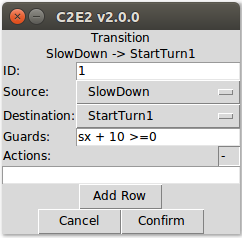
\includegraphics[scale=.25,keepaspectratio=true]{ManualImages/C2E2_version2.0/transition-dialog.png}}
 \caption{Transition Dialog} 
  \label{figure:transition_dialog}
\end{marginfigure}
When adding transition, if you have more than one automaton in your model, one of the automata must be selected - this can be done by right-clicking within the correct automaton, or by having anything in the correct automaton selected when navigating through the menu bar. When editing or deleting transitions, the correct transition must be selected. \\
Transitions do not have names, but rather are defined by their source and destination modes. The source and destination are set by the drop-down menus, which contain all of the modes currently in the automaton. Currently, $\ccee$ supports a singe guard per transition, so if you to include multiple guards, you need to create multiple transitions. Multiple actions are support, and they can be added by clicking the \emph{Add Row} button. 

\section{$\hyxml$ Format}
In this section, we'll review the basics of the $\hyxml$ file format. $\hyxml$ files can be edited directly in $\ccee$ on the \emph{Editor} tab.

\begin{figure}[h!]
\centerline{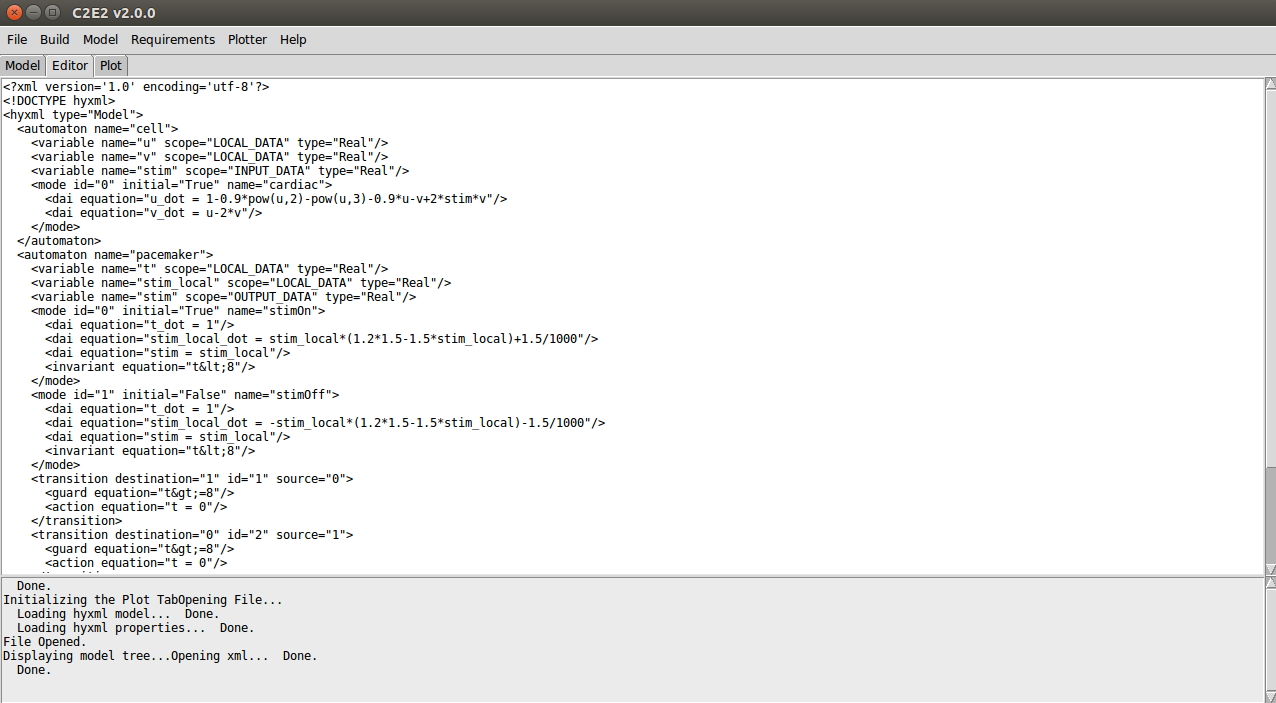
\includegraphics[scale=.22,keepaspectratio=true]{ManualImages/C2E2_version2.0/editor-tab.png}}
\caption{Editor Tab.} 
\label{fig:editor_tab}
\end{figure}

\subsection{Header}
The first few lines of are very familiar to the XML format.\\
\texttt{<?xml version='1.0' encoding='utf-8'?>}\\
\texttt{<!DOCTYPE hyxml>}\\
\texttt{<hyxml type="Model">}\\

\subsection{Automaton}
The first thing we add to our model is an automaton. To add an automaton, use an \texttt{automaton} element, and set it's name with the \texttt{name} attribute. All of our Variables, Modes, and Transitions for this automaton will lie between the opening and closing \texttt{automaton} tags.\\
\vspace{3mm}
\texttt{<automaton name="default\_automaton">}\\
\texttt{</automaton>}

\subsection{Variables}
Next, we add variables to out automaton. To add a varaible, use a \texttt{variable} element, and set it's \texttt{name}, \texttt{scope}, and \texttt{type} attributes.\\
\vspace{3mm}
\texttt{<variable name="sx" scope="LOCAL\_DATA" type="Real"/>}

\subsection{Modes}
Adding mode requires three different elements. The \texttt{mode} element creates the mode and has attributes \texttt{id}, \texttt{initial}, and \texttt{name}. Within an automaton, only one mode can be the initial mode, and mode IDs must be unique.

After adding the opening \texttt{mode} tag, flows and invariants need to be added with the \texttt{dai} and \texttt{invariant} elements, respectively. The \texttt{dai} and \texttt{invariant} elements both have the same single attribute, \texttt{equation}.\\
\vspace{3mm}
\texttt{<mode id="0" initial="True" name="SlowDown">}\\
\texttt{  <dai equation="vx\_dot" = 0.1*ax"/>}\\
\texttt{  <invariant equation="sx + 10 \&lt; 0"/>}\\
\texttt{</mode>}

\subsection{Transitions}

Transitions are similar to modes in the $\hyxml$. First, a \texttt{transition} element must be added. Guards and actions are then added with the \texttt{guard} and \texttt{action} elements, respectively. The \texttt{transition} element has three attributes, \texttt{source}, \texttt{destination}, and \texttt{id}. The \texttt{guard} and \texttt{action} element both have the same single attribute, \texttt{equation}.\\
\vspace{3mm}
\texttt{<transition source="0" destination="1" id="1"}\\
\texttt{  <guard equation="sx + 10 \&gt; = 0">}\\
\texttt{</transition>}


\chapter{Composition, Parsing, and Analysis}
\label{analysis}
In this chapter, we describe in more detail the key operations on hybrid automata that can be performed by $\ccee$. 
The input  a .hyxml file generally contains 
\begin{inparaenum}[(i)]
\item A list of {\em component hybrid automata} $\A_1, \ldots, \A_k$,
\item the definition of (one or more) {\em composed hybrid automaton} $\A$,
\item a list of {\em safety requirements} (See Section~\ref{sec:properties}).
\end{inparaenum}
%
The {$\ccee$} workflow has the following steps: 
\begin{inparaenum}[(i)]
\item 
The component automata $\A_1, \ldots, \A_k$ are  {\em composed\/} according to the definition of the composed automaton $\A$ to generate the complete (internal) representation of $\A$. 
\item 
The automaton model $\A$ is parsed. This generates internal files used for simulation and verification. 
\item Once parsed successfully, $\A$ can be either simulated or verified against the requirements. 
\item Simulations draw random initial states and generate simulation traces and checks for safety of those traces.
\item Verification uses the algorithm presented in~\citet{c2e2:TACAS15,ChuchuATVA} to check the safety property of the give model.
\end{inparaenum}
In the rest of this chapter, we mention some of the key aspects of these four steps.
For details on the mathematical model used here and the algorithms, we refer the reader to~\citet{DuggiralaWMVM14,c2e2:TACAS15}.

\section{Composing}
\label{sec:comp}
It convenient to define a complex model in terms of its components. The composition operation for hybrid automaton defines a bigger (more complex) hybrid automaton $\A$ in terms of a pair of component automata $\A_1$ and $\A_2$. This binary operation can be applied repeatedly to compose a finite set of automata.

A hybrid automaton $\A$ in $\ccee$ is defined by the following following: 
\begin{enumerate}[(i)]
\item $L$: A finite set of {\em modes} or {\em locations}.
\item $X,U,Y$: Finite pair-wise disjoint sets of {\em state (local), input}, and {\em output variables}. State variables are called {\texttt LOCAL} in $\hyxml$.
We will denote the  set of valuations for these variables by $\val{X}, \val{Y}, \val{U},$ etc.
%
%
\item $\D \subseteq L \times L$: A discrete transition graph. For each edge in the graph $(\ell,\ell') \in \D$, two functions are specified. First, $\guard(\ell,\ell'):\val{X} \rightarrow \booleans$ is a {\em transition precondition \/}, and 
$\reset(\ell,\ell'): \val{X} \rightarrow \val{X}$ is a (linear) reset function.
\item $\{f_{\ell}\}$: Differential equations describing the evolution of $X \cup Y$ (with $U$ as input) for each mode $\ell \in L$.
\end{enumerate}
When discussing several automata $\A$, $\A_1$, $\A_2$, etc., we will use subscripts $X_\A, X_1, X_2,$ and $L_\A, L_1, L_2$, etc. to disambiguate components coming from different automata.

For the composition of a pair of hybrid automata $\A_1$ and $\A_2$ to be well-defined, they must be {\em compatible\/}. That is, the following conditions must be met:
\begin{itemize}
    \item $(X_1 \cup Y_1) \cap (X_2 \cap Y_2) = \emptyset$,
    \item $U_1 \subseteq Y_2$ and $U_2 \subseteq Y_1$ 
\end{itemize}
In the current implementation of $\ccee$, $\A_1$ and $\A_2$ can only interact through shared variables, and not through shared transitions.

For a pair of compatible automata $\A_1$ and $\A_2$ the {\sf Compose\/} operation of $\ccee$, constructs the composed automaton $\A$ (as defined below). Once this composed model is saved, a new $\hyxml$ file with the composed automaton is saved.

%as defined in~\cite{TIOAmon,Mitra07PhD}:
\begin{enumerate}[(i)]
\item $L_\A = L_1 \times L_2$,
\item $X_\A = X_1 \cup X_2$,
$Y_\A = Y_1 \cup Y_2$,
$U_\A = \emptyset$.
%%
%
\item $((\ell_1,\ell_2),(\ell_1',\ell_2')) \in \D_\A$ iff 
$(\ell_1,\ell_1') \in \D_1$ and $\ell_2 = \ell_2'$, or \\
$(\ell_2,\ell_2') \in \D_2$ and $\ell_1 = \ell_1'$.
%
\item $\{[f_{1,\ell_1}; f_{2,\ell_2}]\}$ 
for each mode $(\ell_1,\ell_2) \in L_\A$, the differential equations for $X_\A = X_1 \cup X_2 \cup Y_1 \cup Y_2$, are derived by simply concatenating the differential equations for 
$(X_1 \cup Y_1)$ in mode $\ell_1$ with those for $(X_2 \cup Y_2)$ in mode $\ell_2$.
%
The differential equations for each mode of $\A$ are derived from those of the component modes. 
\
\end{enumerate}




%\sayan{In section 10, we should have one simple example with composition.}

\section{Parsing}

Before any simulation or verification can happen, the system must first be parsed. When parsing, we perform a variety of checks to make sure the system is capable of being simulated and verified. 
In the following sections we enumerate these checks (see Section~\ref{sec:editing} for details about the $\hyxml$ format).


    \subsection{Variables}
        \begin{itemize}
            \item Local variables must all be distinct from all other variables in the model
            \item Output variables must be distinct from all local variables
            \item Output variables must be distinct from all other output variables
            \item Input variables must be distinct from all local variables
            \item Input variables must be distinct from other input variables within the same automaton
            \item Every input variable must have a matching output variable in a different automaton
        \end{itemize}
    \subsection{Mode}
        Mode names and mode IDs must be unique within an automaton. Note that mode IDs can only be changed through editing the $\hyxml$ directly. 
        \subsection{Flows}
            \begin{itemize}
                \item Expressions must be standard mathematical expressions and use standard mathematical operators
                \item Expression contains only one symbol on the left-hand side
                \item Output variables on right-hand side must not end with \_dot
                \item Local variables on left-hand side must end with \_dot
                \item Input variables must not be used on the left-hand side
            \end{itemize}
        \subsection{Invariants}
            \begin{itemize}
                \item Expressions must be standard mathematical expressions and use standard mathematical operators. 
            \end{itemize}
    \subsection{Transition Guards}
            \begin{itemize}
                \item Expressions must be standard mathematical expressions with standard mathematical operators. 
                \item Expressions must be separated by "\&\&". 
            \end{itemize}
        \subsection{Transition Actions}
            \begin{itemize}
                \item Expressions must be standard mathematical expressions with standard mathematical operators.
                \item Expressions must be separated by "\&\&".
            \end{itemize}


%\sayan{Compatibility checks. This happens here or in compose?}

%List of error messages and their interpretations.


\section{Simulation}\label{sec:simulation}

When the {\sf Simulate} button is clicked, $\ccee$  transforms the input hybrid automaton model and  generates faithful numerical simulations of this model.
The type of simulator used can be chosen by the user. The most robust simulator is {\sf ODEInt} from the {\sf Boost} library. 
%
Other validated numerical simulators like {\sf VNODE-LP}~\citet{vnode2006} and {\sf CAPD} are also supported but because of numerical instability issues, using these simulators may  require some extra work in the latest version of $\ccee$. 
%

Roughly, the simulation procedure works as follows.
A sequence of initial states are drawn randomly from the specified starting set. 
From each of these initial states, a simulation in the current mode is generated using the C++ simulator function. This function is compiled when the $\hyxml$ file is parsed. 
Once the simulation in the current mode is computed, the result is  checked to see if any guards are hit.
If any of the guards are hit, the simulation is truncated, the initial state in the next mode is computed using the reset function, and the simulation is continued in the new mode for the remaining time. 
If none of the guards are hit, the simulation is complete.
This procedure is repeated for all the initial state. 
If any of the simulations hit the specified ``unsafe set'', then the result unsafe is returned, otherwise the result ``safe'' is returned. Of course, ``safe'' does not mean that all behaviors from the starting set are safe. 
%
The  simulation output is stored in a text file in the working directory.


\section{Verification}\label{sec:verification}
%
%    \item We start by generating a cover of the initial set by partitioning our initial set into smaller regions
%\item Next, we simulate the center point of each cover
%\item Once the simulation is compute, we read the result and check to see if any guards are it.
%\item If any of the guards are hit, we truncate the simulation where that happened, then run the simulation making the appropriate transition.
%\item If none of the guards are hit, the simulation is complete.
There are several papers describing the $\ccee$ verification algorithms~\citet{ChuchuATVA,fan2016automatic,DMVemsoft2013,fan2016automatic,DuggiralaWMVM14} and therefore we are not going to repeat them here. 
%
For linear systems a global discrepancy function is used, while for nonlinear systems the local discrepancy computation presented in~\citet{ChuchuATVA,FanKJM18} is implemented.  
% 
The reach tubes computed for verification are stored in a textfile in the working directory.
%

You may want to look at some of the applications of $\ccee$ in verification of cyber-physical systems:
Toyota's Powertrain control system~\citet{DuggiralaFM015},
NASA landing alarm system~\citet{DuggiralaWMVM14}, 
Complex transistor models~\citet{FanM0BM018},  model of cardiac pacemaker~\citet{HuangFMMK14,HuangFMMK15}, and autonomous spacecraft maneuvers~\citet{ChanM17}.
%
Several other examples are reported in the ARCH competition of 2018~\cite{AlthoffB0FFFKLM18}.
We will be happy to hear about your applications; send email to  \href{mailto:c2e2help@gmail.com}{c2e2help@gmail.com}. 

\chapter{Plotter}

{$\ccee$} version 2.0 comes with a completely overhauled plotter. On the new \emph{Plot} tab, you can plot any data set you choose, and the result will be an interactive HTML plot that you can use to focus in on certain parts of your data.

The \emph{Plot} tab has two main components - the \emph{plot pane}, where small images on the plots are displayed, and the \emph{plot sidebar}, where plots can be created and edited.

\begin{figure}[h!]
\centerline{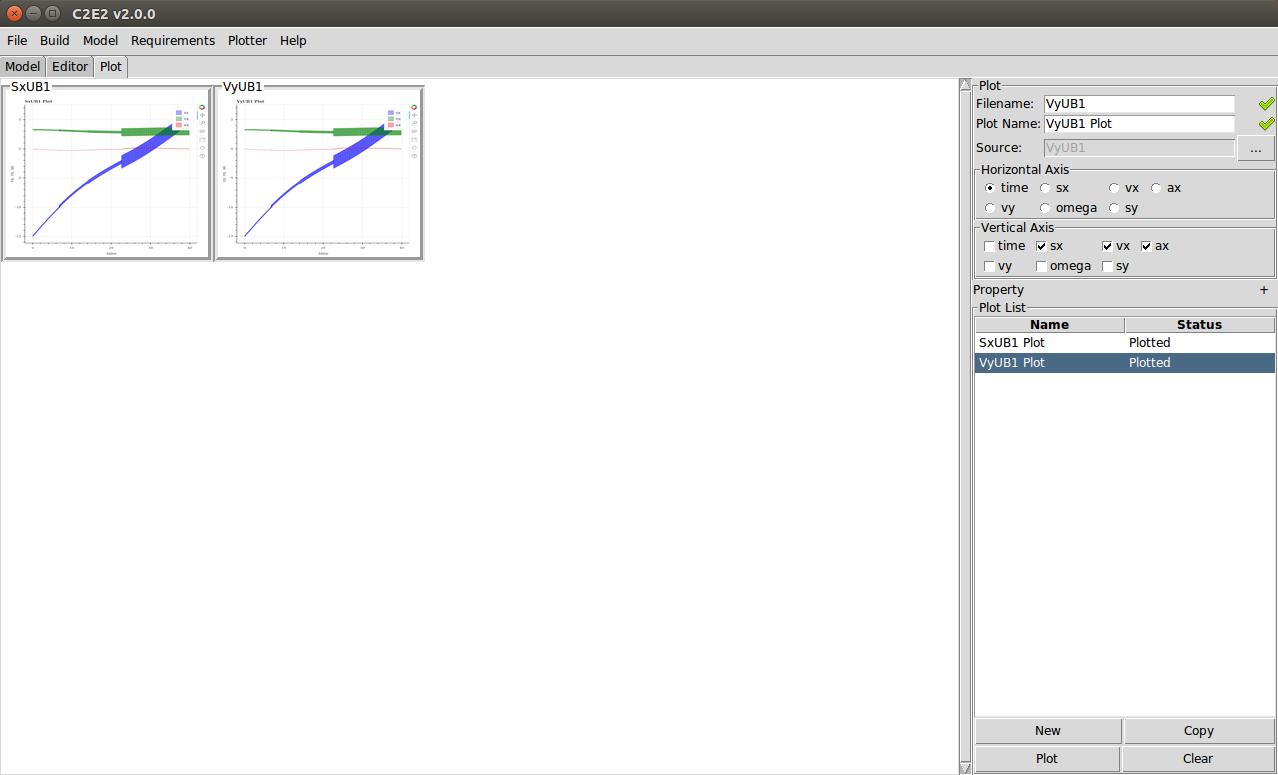
\includegraphics[scale=.22,keepaspectratio=true]{ManualImages/C2E2_version2.0/plot-tab.png}}
\caption{Plot Tab.} 
\label{fig:plottab}
\end{figure}

\section{Creating and Editing Plots}

To create a plot, the first thing you need to do is select the data source. To do this, select on the button next to the \emph{Source} field (labeled "..."), and choose which file to load - the data files generated by $\ccee$ are stored in the \texttt{/work-dir/output/} directory. As mentioned, this can be any data source generated by $\ccee$, it does not have to be related to the model you currently have open in the \emph{Model} and \emph{Editor} tabs. Next, fill out the \emph{Filename} and \emph{Plot Name} fields.

\begin{itemize}
    \item Filename\\
        This represents the filename used to store the various plots generated by the plotter. Two files will be generated using this name, \emph{filename}.html and \emph{filename}.png. The PNG file is the preview image displayed done the \emph{plot pane}, and the HTML file in the interactive plot. 
    \item Plot Name\\
        This the title as it will be displayed on your plot.
    \item Source\\
        This is the data source used to create the plot. The data source used must be a properly-formatted file generated by $\ccee$ when running a simulation or verification. These files will be stored in the \texttt{/work-dir/output/} directory and be named after the requirement that created them.
\end{itemize}

If you recently simulated or verified a requirement, you may notice that you have this field, as well as plot name and file name, already filled out. This is because $\ccee$ automatically creates a new plot with the fields defaulted in when a requirement is simulated or verified. 

Next, you need to choose which variables will appear on the vertical axis, and which will appear on the horizontal axis. You can only select one variable to be on the horizontal axis, and you must choose at least one variable to be on the vertical axis. 

Finally, click on the \emph{Plot} button. Once the plotting is complete, you will see a preview appear on the \emph{plot pane}. You can double-click on this image to open the interactive HTML plot in your default browser.

\section{Multiple Plots}

Multiple plots can be added by using the \emph{New} and 
\emph{Copy} buttons, and they will be displayed in the \emph{Plot List} on the \emph{Plot Sidebar}. 

\section{Requirements}
\begin{marginfigure}
 \centerline{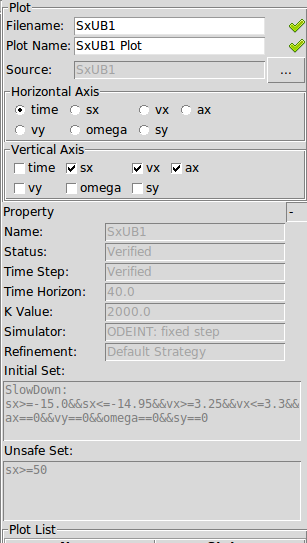
\includegraphics[scale=.25,keepaspectratio=true]{ManualImages/C2E2_version2.0/plot-properties.png}}
 \caption{Requirements Display} 
  \label{figure:requirements_display}
\end{marginfigure}

The requirements (properties) that were used to create the source data file can be displayed by clicking on the + next to the \emph{Properties} label.





% \chapter{Plotter}
% \label{sec:plots}

% Once the verification of a property is complete, $\ccee$ will also launch a plotter panel for each verified property with the name $\langle$\texttt{property name}$\rangle$ \texttt{plot}. Double click on the properties can also open a new tab as the plotting panel for the property. This is the plotting window for this property: it enables us to plot various projections of the reach set that has been computed in verifying the property. 
% \begin{figure}[!htbp]
%  \centerline{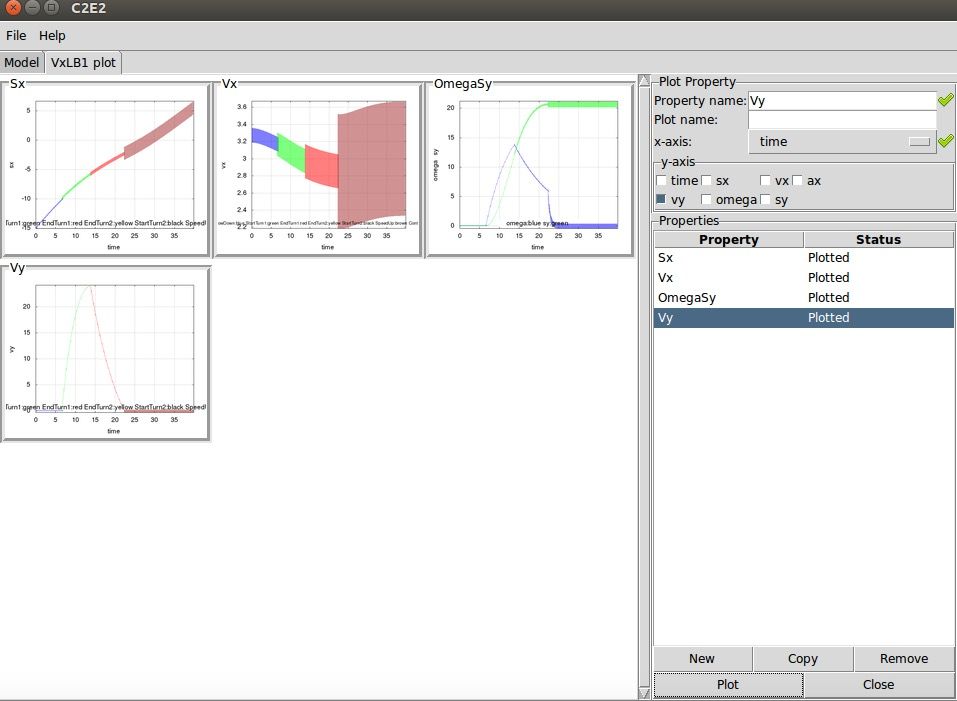
\includegraphics[scale=.25,keepaspectratio=true]{./Manual_ver0_3_image/plotter_result.png}}
%  \caption{The plotting tab for property 1 without any plots.} 
% \end{figure}
% %
% \newline
% The plot window has two parts. 
% The left pane shows all the plots icons and the right pane is used to create new plots. 
% The steps for creating new plots (as in Figure~\ref{fig:plot_dialog}) is similar to that for creating properties:  
% \begin{enumerate}
% \item Click \texttt{New} right bottom corner of the window. This enables editing a new plot. Note here we are slightly abusing the name by calling different plots different \textit{properties}.
% \item Enter a name for the plot, say \texttt{Vy}, in \texttt{Property name} textbox at the right top of the panel.
% \item The \texttt{Plot name} textbox is an option to give the plots the title names.
% \item Select the x-axis and y-axis variables below the property name, and add more y-axis variable if needed. You can plot a state variable with respect to time (for example, x vs. t) or two state variables (x vx. y).
% You can also plot multiple state variables with respect to time (x and y vs. t). 
% \item Click the \texttt{Plot} button.
% \end{enumerate}



% \begin{marginfigure}
%  \centerline{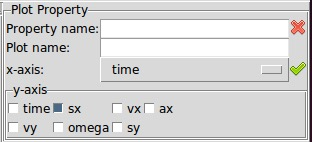
\includegraphics[scale=.24,keepaspectratio=true]{Manual_ver0_3_image/plotter_dialog.png}}
%  \caption{Add Plot dialog box.} 
%  \label{fig:plot_dialog}
% \end{marginfigure}


% %
% $\ccee$ can currently create two dimensional plots as Figure~\ref{fig:reachtube_plot}. As before, you can add more plots or copy/remove/plot multiple plots. 

% %When you add/edit the plots, you will see a dialog box where you can select the variables would like to plot.


% %Once you are satisfied with your plots, you can click the plot button generate the plots. 


% As the program plots the reach sets, you will see icons appear on the left hand side of the window with a preview of what the plot looks like as well as the plot name below it. You can expand the plot by double clicking on these icons. All generated figures of the plot  are stored in the work-dir/plotresult folder.
% %The plot window allows you to pan and zoom over the reach tube and also 

% You can navigate to the first window and other opened plot windows by clicking on the tabs along the upper portion of the window. You can save the model as well as the properties you have created in an \texttt{.hyxml} file. 


% %Clicking on the \texttt{Plot} button will create 
% %the plots one by one and show the resulting icons.





% \begin{marginfigure}
%  \centerline{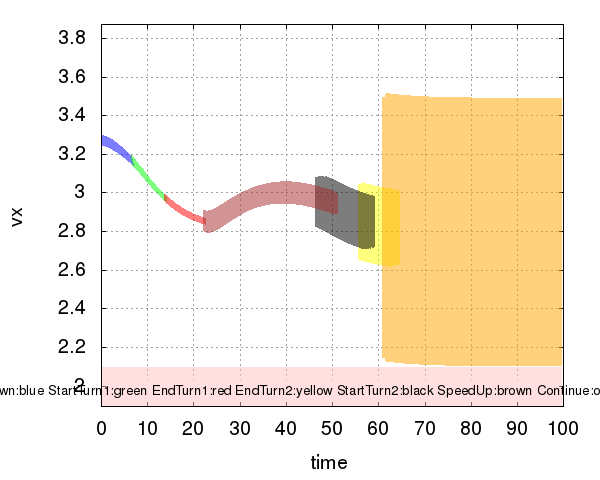
\includegraphics[scale=.24,keepaspectratio=true]{Manual_ver0_2_image/plot_open.png}}
%  \caption{A plot of a reach tube of one variable with respect to time.} 
%  \label{fig:reachtube_plot}
% \end{marginfigure}

% \subsection{Plots with multiple variables and modes}
% \label{sec:multiplots}

% If plotting multiple variables on the y-axis, the reach tube of each variable will be shown in different colors with labels. For example, in Figure~\ref{fig:xytime} the $x$-axis is time and the $y$-axis shows the reach tubes of two variables $\omega$ and $v_x$ which are shown in blue and green respectively. The axis for $v_x$ is labeled by green and that of $\omega$ is labeled by blue.

% \begin{marginfigure}
%  \centerline{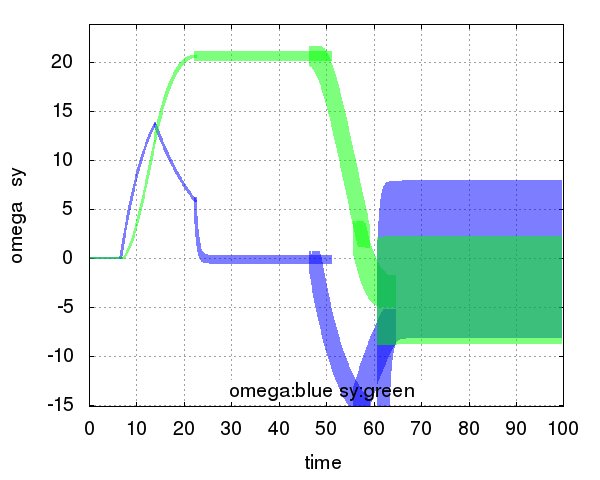
\includegraphics[scale=.24,keepaspectratio=true]{Manual_ver0_2_image/PLOT_RESULT_DOUBLE.png}}
%  \caption{A plot of a reach tube of two variables with respect to time.} 
% \label{fig:xytime}
% \end{marginfigure}

% \section{Loading and Saving}
% \label{sec:loadsave}

% Currently $\ccee$ provides very basic functionality for loading and saving models and properties. 
% You can save a model and its properties from the file menu. 
% The saved file is in the \texttt{.hyxml} format as shown below~\citet{SM:HSCC2011}.
% Once saved, a model and the properties in the \texttt{.hyxml} file can be loaded from the file menu.

% Changes made to the model in the $\ccee$ front end are {\bf not\/} saved but only the edited properties are saved.
% However, you can edit the \texttt{.hyxml} file using a text editor to change the model and the properties.
% The reach sets computed during verification are stored in the working directory \texttt{/work-dir/} but currently they cannot be loaded.

\chapter{Command-Line Interface}

$\ccee$ allows a limited number of its functions to be used fromm the command-line without launching the GUI. In brief, it allows an existing $\hyxml$ model to be simulated and verified, and the results to be stored in appropriate files. The GUI has to be used for model editing and plotting. 


In the $\ccee$ folder, type command ./runC2E2command to launch the command-line version of $\ccee$ and you should able to see the model list (as in Figure~\ref{figure:terminalmain}). Command line version of $\ccee$ can only read models in the \texttt{Examples} folder. If you have customized models, please place them in the \texttt{Examples} folder as well. 
 \begin{marginfigure}
  \centerline{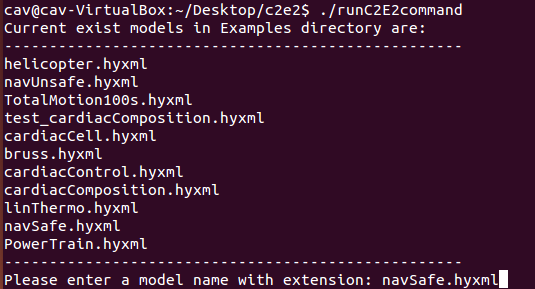
\includegraphics[scale=.15,keepaspectratio=true]{Manual_ver0_2_image/terminal_main.png}}
  \caption{Command line version $\ccee$ interface} 
   \label{figure:terminalmain}
 \end{marginfigure}

% \newline

 Once you load a file, $\ccee$ will start to compile the simulator, and it will ask you to identify if it is a linear model or nonlinear model (see Figure~\ref{figure:terminallinear}). Type Y or N to answer, then the model will be successfully loaded.
  \begin{marginfigure}
  \centerline{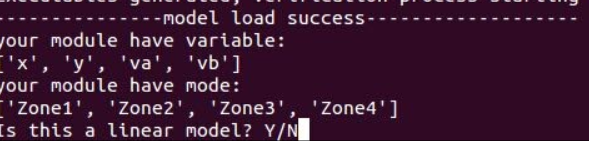
\includegraphics[scale=.15,keepaspectratio=true]{Manual_ver0_2_image/terminal_linear.png}}
  \caption{Type Y or N to tell $\ccee$ if the model is linear.} 
   \label{figure:terminallinear}
 \end{marginfigure}

Once the model is loaded, there will be various of commands you can use. Type \texttt{help} command to check the all the commands (see Figure~\ref{figure:terminalhelp}). These commands are similar to the functionality we have described in Section \ref{sec:open}. To check the properties that come with the \texttt{.hyxml} file, type \texttt{printprop} command. This command will expand all the built in properties as shown.By typing the \texttt{verify} command, you can verify all the properties in the property list. Results will be shown once the verification ends as in Figure~\ref{figure:terminalverify}.
 \begin{marginfigure}
  \centerline{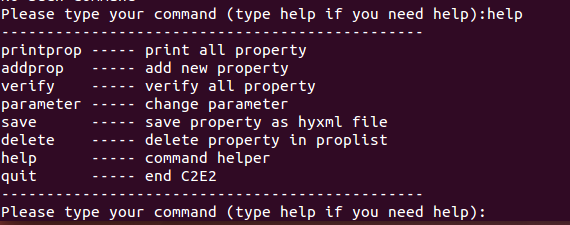
\includegraphics[scale=.25,keepaspectratio=true]{Manual_ver0_2_image/terminal_help.png}}
  \caption{All command-line options.} 
   \label{figure:terminalhelp}
 \end{marginfigure}

% When you are finishing with the command line version $\ccee$, you can type \texttt{quit} command to exit.







% \begin{figure}
%  \centerline{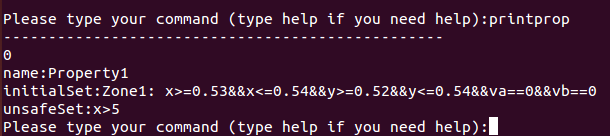
\includegraphics[scale=.25,keepaspectratio=true]{Manual_ver0_2_image/terminal_prop.png}}
%  \caption{Expand properties come with the model \texttt{.hyxml} file.} 
%   \label{figure:terminalprop}
% \end{figure}

 \begin{marginfigure}
  \centerline{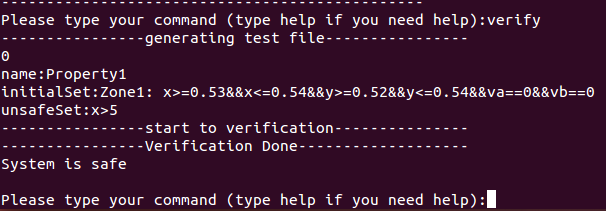
\includegraphics[scale=.25,keepaspectratio=true]{Manual_ver0_2_image/terminal_verify.png}}
  \caption{Verify the properties in the property list.} 
   \label{figure:terminalverify}
 \end{marginfigure}

\chapter{Building models for $\ccee$}
\label{sec:plots}
In this chapter, we will discuss two example $\ccee$ models. 


% \section{Format of HyXML}
% \label{sec:hyxml}
% Currently, $\ccee$ only accepts models of a certain form. The model can be defined in the HyXML file format - many examples of this can be found in the Examples/ directory. Multiple attributes must be defined for it to be a valid model. The attributes marked by * must be defined but are not used currently.
% \begin{itemize}
% \item The root layer should be \textit{<hyxml type="Model">} ending with \textit{</hyxml>}
% \item automaton with name
% 	\begin{itemize}
% 	\item variable
%     	\begin{itemize}
% 		\item name
% 		\item scope $\rightarrow$ LOCAL\_DATA, INPUT\_DATA, OUTPUT\_DATA
% 		\item type* $\rightarrow$ Real, Integer
%         \end{itemize}
% 	\item mode (unique id's, consecutive order - 0 to n)
%     	\begin{itemize}
%         \item id
% 		\item initial $\rightarrow$ True, False
%         \item name
% 		\item dai $\rightarrow$ An equation of the form v\_dot = algebraic formula if v is a local variable, else v\_out = algebraic formula if v is an output variable
% 		\item invariant $\rightarrow$ Equation must be linear and use only local variables (Use \&lt; for <, etc)
% 		\end{itemize}
% 	\item transition
%     	\begin{itemize}
% 		\item source, destination $\rightarrow$ IDs of modes
% 		\item id* $\rightarrow$ id of transition
% 		\item guard $\rightarrow$ Equation must be linear and use only local variables (Use \&lt; for <, etc)
% 		\item action (optional) $\rightarrow$ Can only use local variables and must be of the form v = linear formula
%         \end{itemize}
%     \end{itemize}
% \item composition $\rightarrow$ automata should be a semicolon separated list of automata names you are composing
% \item property
% 	\begin{itemize}
% 	\item unsafeSet $\rightarrow$ Conjunction of linear inequalities
% 	\item initialSet $\rightarrow$ <mode\_name>: Conjunction of linear inequalities
% 	\item name $\rightarrow$ verification/simulation data can be found at wd/ReachSet<name>
% 	\item parameters
%     	\begin{itemize}
% 		%\item taylororder $\rightarrow$ Taylor terms you want in the expansion
% 		\item timestep $\rightarrow$ Only used in ODE\_FIXED and CAPD
% 		\item timehorizon $\rightarrow$ Length of time you want to simulate for
% 		\item Kvalue
%         \end{itemize}
%     \end{itemize}
% \end{itemize}



\section{Example 1: Laub-Loomis}
\label{sec:exp1}
The first example mentioned is a continuous system with nonlinear dynamics. The example we used is the Laub-Loomis model. It is a model with seven variables. The dynamics of the model is given by.
\[
\left\{
\begin{array}{lcl}
 \dot{x}_1 & = & 1.4x_3 - 0.9x_1 \\
 \dot{x}_2 & = & 2.5x_5 - 1.5x_2 \\
 \dot{x}_3 & = & 0.6x_7 - 0.8x_2x_3 \\
 \dot{x}_4 & = & 2 - 1.3x_3x_4 \\
 \dot{x}_5 & = & 0.7x_1 - x_4x_5 \\
 \dot{x}_6 & = & 0.3x_1 - 3.1x_6 \\
 \dot{x}_7 & = & 1.8x_6 - 1.5x_2x_7
\end{array}
\right.
\]


In this example, we use initial set given by $x_1(0)\in[1.1,1.3]$, $x_2(0)\in[0.95,1.15]$, $x_3(0)\in[1.4,1.6]$, $x_4(0)\in[2.3,2.5]$, $x_5(0)\in[0.9,1.1]$, $x_6(0)\in[0,0.2]$, $x_7(0)\in[0.35,0.55]$, and the unsafe set is $x_4\leq5$.
The model is running in time interval $t\in[0,20]$. The problem can be described as follows.
%\sayan{Had to comment this out.}

\lstinputlisting[language=XML]{Examples/Laub-Loomis.hyxml}

$\ccee$ is able to solve the model with time step 0.05 and k is set to be 50. The computed reachtube for variable $x_4$ is shown in Figure~\ref{plot:laubloomis}.


\begin{marginfigure}
\centerline{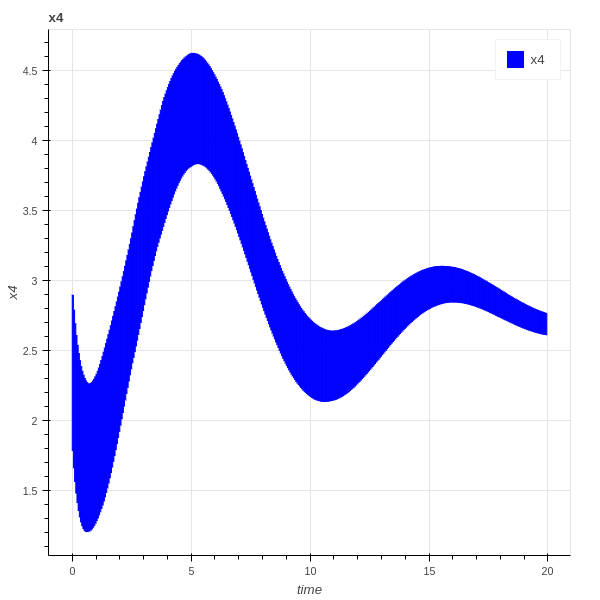
\includegraphics[scale=.24,keepaspectratio=true]{Examples/laublarge.png}}
 \caption{Plot for $x_4$ for example 1.} 
 \label{plot:laubloomis}
\end{marginfigure}

\pagebreak

%blah 
\section{Example~2: Cell and Pacemaker}
\label{sec:secondex}

The second example mentioned is a hybrid system. The example we used is the FitzHugh-Nagumo (FHN) model. The model has 2 variables and 2 modes. The dynamic for each mode is give by hybrid automaton. \\

In this example, we use initial set given by $u(0)=0$ and $v(0)=0$ and a variable t is introduced to track time spend in each mode. The model is running in time interval $t\in[0,40]$. The problem can be described as follows.

\vspace{1cm}
\tikzset{
    state/.style={
           rectangle,
           rounded corners,
           draw=black, very thick,
           minimum height=2em,
           inner sep=2pt,
           text centered,
           },
}

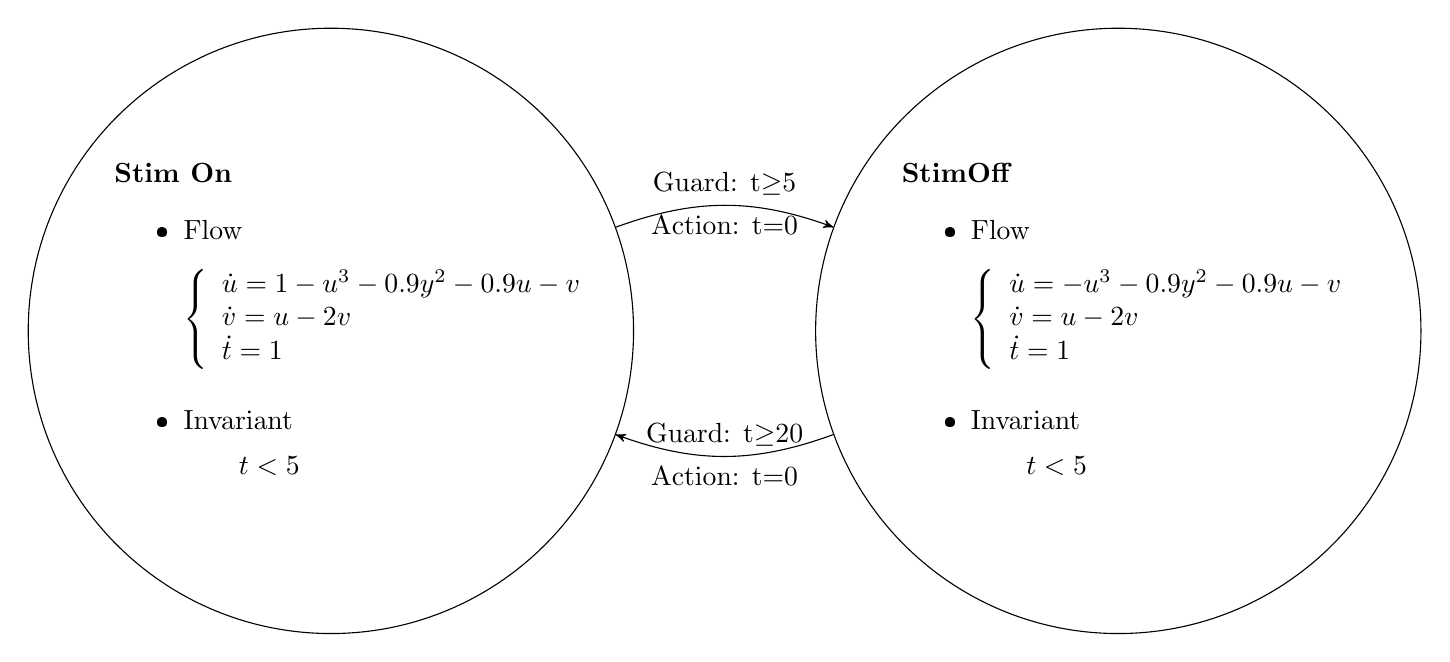
\begin{tikzpicture}[->,>=stealth']

 % Position of QUERY 
 % Use previously defined 'state' as layout (see above)
 % use tabular for content to get columns/rows
 % parbox to limit width of the listing
 \node[state] (StimOn) 
 {\begin{tabular}{l}
  \textbf{Stim On}\\
  \parbox{5.5cm}{\begin{itemize}
   \item Flow
   \[
\left\{
\begin{array}{lcl}
 \dot{u}  =  1-u^3-0.9y^2-0.9u-v \\
 \dot{v}  =  u-2v\\
 \dot{t}  =  1 \\
\end{array}
\right.
\]
   \item Invariant
    \subitem $t<5$
   \end{itemize}}
 \end{tabular}};
  
 % State: ACK with different content
 \node[state,    	% layout (defined above)
  right of=StimOn, 	% Position is to the right of QUERY
  node distance=10cm, 	% distance to QUERY
  anchor=center] (StimOff) 	% posistion relative to the center of the 'box'
 {%
 \begin{tabular}{l} 	% content
  \textbf{StimOff}\\
  \parbox{5.5cm}{\begin{itemize}
   \item Flow
      \[
        \left\{
        \begin{array}{lcl}
        \dot{u}  =  -u^3-0.9y^2-0.9u-v \\
        \dot{v}  =  u-2v \\
        \dot{t}  =  1
        \\
        \end{array}
        \right.
      \]
   \item Invariant    
   \subitem $t<5$
   \end{itemize}}
 \end{tabular}
 };
 


 % draw the paths and and print some Text below/above the graph
 \path (StimOn) edge[bend left=20]  node[anchor=south,above]{Guard: t$\geq$5} node[anchor=south,below]{Action: t=0}(StimOff);
 
 \path (StimOff) edge[bend left=20] node[anchor=north,above]{Guard: t$\geq$20} node[anchor=north,below]{Action: t=0}(StimOn);

\end{tikzpicture}



\lstinputlisting[language=XML]{Examples/cardiacComp.hyxml} %TODO: fix included code
$\ccee$ is able to solve the model with time step 0.01 and k value 2000. The computed reachtube for variable v is shown in Figure~\ref{plot:cardiac}

\begin{marginfigure}
%	\vspace{6cm}
\centerline{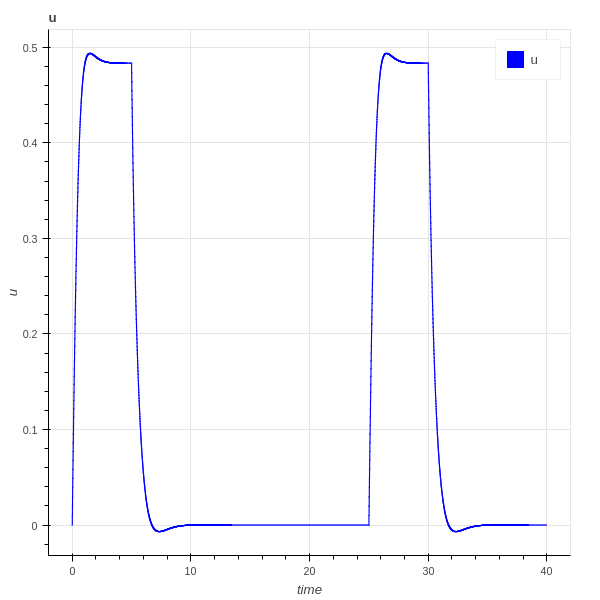
\includegraphics[scale=.24,keepaspectratio=true]{Examples/cardiacu.png}}
 \caption{Plot for $u$ for example 2} 
 \label{plot:cardiac}
\end{marginfigure}

\section{Intermediate Files}
\label{sec:pnf}
Several files are generated while verifying the model and some of them are worth mentioning.
\paragraph{jacobiannature1.txt}
The \textit{jacobiannature1.txt} file contains the jacobian for the dynamic of the system. If the system have multiple modes, files with higher index will be generated and each file correspond to one mode of the system. Each file contain the number of variables, the name of variables, the total number of entries in the jacobian matrix and the matrix itself. These files are used in computing the reach tube.
\paragraph{simulator.cpp}
The \textit{simulator.cpp} file is auto generated by the frontend. It contains a simulator for the model for simulation engine odeint. The file can be compiled to an independent executable \textit{simu} which is also located inside the work-dir folder. The simulator \textit{simu} and it's corresponding configuration file \textit{Config} (which is also located in work-dir folder), can be executed and providing simulation result by using commnad "./simu < Condig".
\paragraph{SimuOutput}
The \textit{SimuOutput} file contains the simulated result for the model. 
\paragraph{reachtube.dat}
The \textit{reachtube.dat} file contains the computed reach tube for the model.

\appendix

\chapter{Required Libraries}
\label{app:packs}
The following is a complete list of packages needed for installing $\ccee$. 
\begin{enumerate}
 \item GNU Linear Programming Kit along with Python bindings, GLPK and PyGLPK (http://www.gnu.org/software/glpk/) (http://tfinley.net/software/pyglpk/)
 \item GNU parser generator, Bison (http://www.gnu.org/software/bison/)
 \item The Fast Lexical Analyzer, Flex (http://flex.sourceforge.net/) 
 \item Python (http://www.python.org/)
 \item Python parsing libraries, Python-PLY (http://code.google.com/p/ply/)
 \item GTK libraries for Python (http://www.pygtk.org/)
 \item Plotting libraries for Python, Matplotlib (http://matplotlib.org/)
 \item Packing configurations library  (http://www.freedesktop.org/wiki/Software/pkg-config/)
 \item GNU Autoconf (http://www.gnu.org/software/autoconf/)
 \item Python xml library, lxml (http://lxml.de/installation.html)
 \item Parma Polyhedron Library (http://bugseng.com/products/ppl/)
 \item Python Sympy library (http://www.sympy.org/en/index.html)
 \item Boost libraries (http://www.boost.org)
 \item Python Numpy library (http://www.numpy.org/)
 \item Python SciPy library (https://www.scipy.org/)
 \item Python Pillow library (https://python-pillow.org/)
 \item Python3 GnuPlot library (https://github.com/oblalex/gnuplot.py-py3k)
\end{enumerate}

% If you get any errors while installing PyGLPK, please visit the following website:\\ \url{http://tfinley.net/software/pyglpk/building.html} and install it manually.

\backmatter

%----------------------------------------------------------------------------------------
%	BIBLIOGRAPHY
%----------------------------------------------------------------------------------------

\bibliography{sayan1} % Use the bibliography.bib file for the bibliography

\bibliographystyle{plainnat} % Use the plainnat style of referencing

%----------------------------------------------------------------------------------------

\printindex % Print the index at the very end of the document

\end{document}